\chapter{Background}
\section{Transformer Language Models}

The Transformer architecture, introduced by Vaswani et al. \cite{vaswani_attention_2017}, revolutionised natural language processing and other fields. In contrast to conventional sequence-to-sequence models that depend on recurrent or convolutional layers, Transformers leverage self-attention mechanisms to comprehend connections among tokens within a sequence. 

There are conventionally three variants of transformer language models:
\begin{itemize}
    \item \textbf{Decoder-only} models, such as GPT-3 \cite{brown_language_2020}, autoregressively produce embeddings of the input sequence from which the next token is generated.
    \item \textbf{Encoder-only} models, such as BERT \cite{devlin_bert_2019}, produce embeddings of the input sequence by encoding the input sequence bi-directionally.
    \item \textbf{Encoder-Decoder} models, such as T5 \cite{raffel_exploring_2020}, transform an input sequence into an embedding via the encoder, which the decoder then uses to generate an output sequence autoregressively.
\end{itemize}

We focus on autoregressive decoder-only models due to their popularity and success.

\section{Decoder-only Models}
The model begins by processing a sequence of input tokens $\bm{t}$ of length $n$ one-hot encoded through an embed layer with embedding matrix $W_E$ of dimensionality $({|\mathcal{V}|\times d})$ where $\mathcal{V}$ is the set of vocabulary and $d$ is the dimensionality of an embedding. This results in a sequence of embeddings $x$ of length $n$ with each embedding of dimensionality $d$. Or $\bm{X}$ with dimensions $({n \times d})$, which maps them into a continuous vector space \cite{ferrando_primer_2024}. The next part of the architecture consists of a sequence of residual blocks, each comprising an attention layer followed by a multilayer perceptron (MLP) layer. Within each residual block, the attention and MLP layers access the residual stream by applying linear projections to their inputs. These layers' outputs are subsequently integrated into the residual stream through additive linear projections. Each block's attention mechanism comprises multiple attention heads that function in parallel, capturing different aspects of the input dependencies. The final stage of the model involves a token unembedding process, which converts the processed representations back into the token space through unembedding matrix $W_U$ with dimensionality $({d \times |\mathcal{V}|})$.

\begin{figure}[ht]
    \centering
    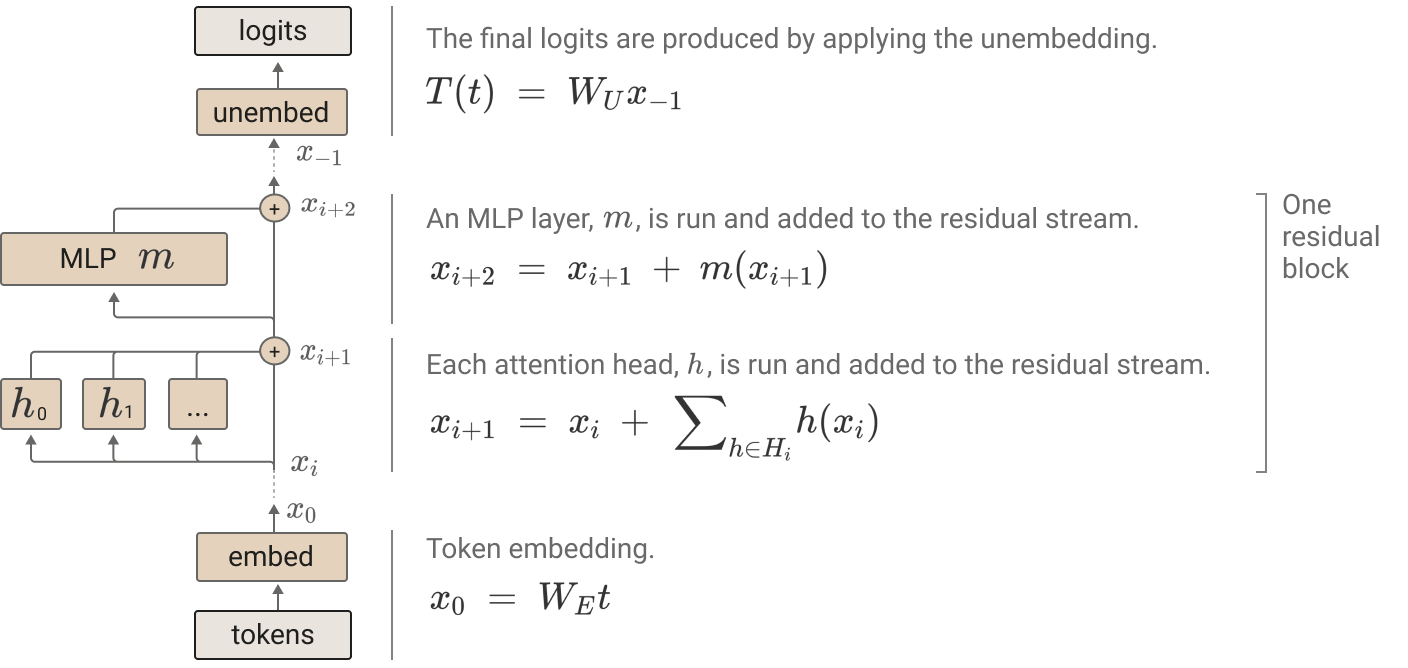
\includegraphics[width=1\textwidth]
    {transformer_architecture.png}
    \caption{High-level architecture diagram of a transformer model \cite{nanda_mathematical_nodate}}
    \label{fig:enter-label}
\end{figure}

\newpage
\subsection{Attention}
The attention mechanism is a crucial innovation in transformer architectures for contextualizing token representations at each layer. Attention allows the model to dynamically focus on and combine relevant information from different parts of the input sequence. This capability is essential for tasks requiring an understanding of word relationships, handling long-range dependencies, and capturing contextual meaning in language.

\begin{figure}[h]
    \centering
    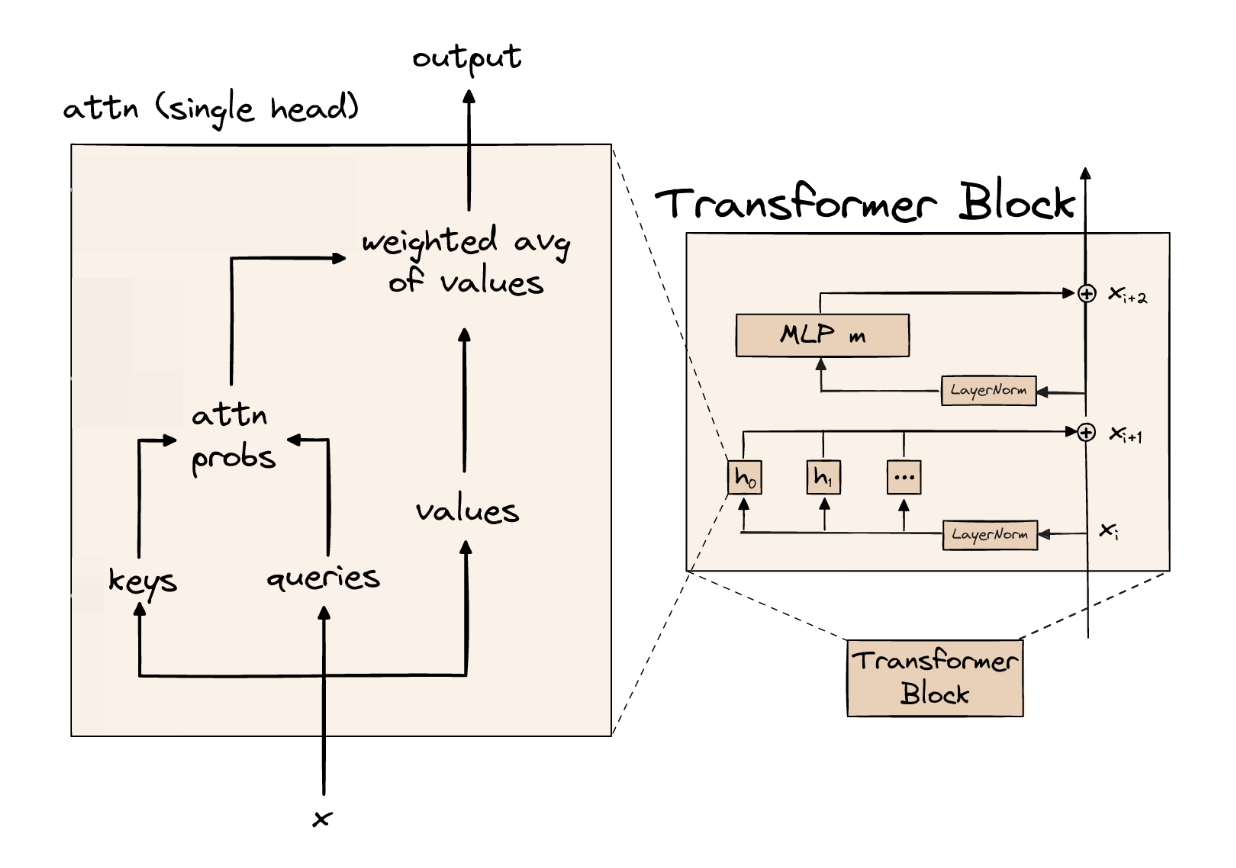
\includegraphics[width=0.85\linewidth]{attention.png}
    \caption{Attention head details \cite{colab_transformer_2024}}
\end{figure}

As our model is autoregressive, when decoding token $i$, the attention head will only read values from the residual stream for positions $<=i$, anything after is masked as a token can only see the context that comes before it.

Through specialized attention heads, the model can perform various functions like processing syntactic relationships, joining subwords, and handling positional information.

\subsection{MLP}
While attention handles interactions between tokens, MLP blocks process each token's representation independently. They act as the model's primary mechanism for storing and accessing learned information.

The MLP is a standard FFN with a singular hidden layer and a non-linear activation function \cite{ferrando_primer_2024}. We first have two learnable weight matrices which are $W^l_{in}$ with dimensionality $(d \times d_{mlp})$ and $W^l_{out}$ with dimensionality $(d_{mlp} \times d)$ where the intermediate value is passed through a non-linear activation function, so:
$$MLP^l(x_i^l) = g(x_i^lW_{in}^l)W_{out}^l$$

\begin{figure}[h]
    \centering
    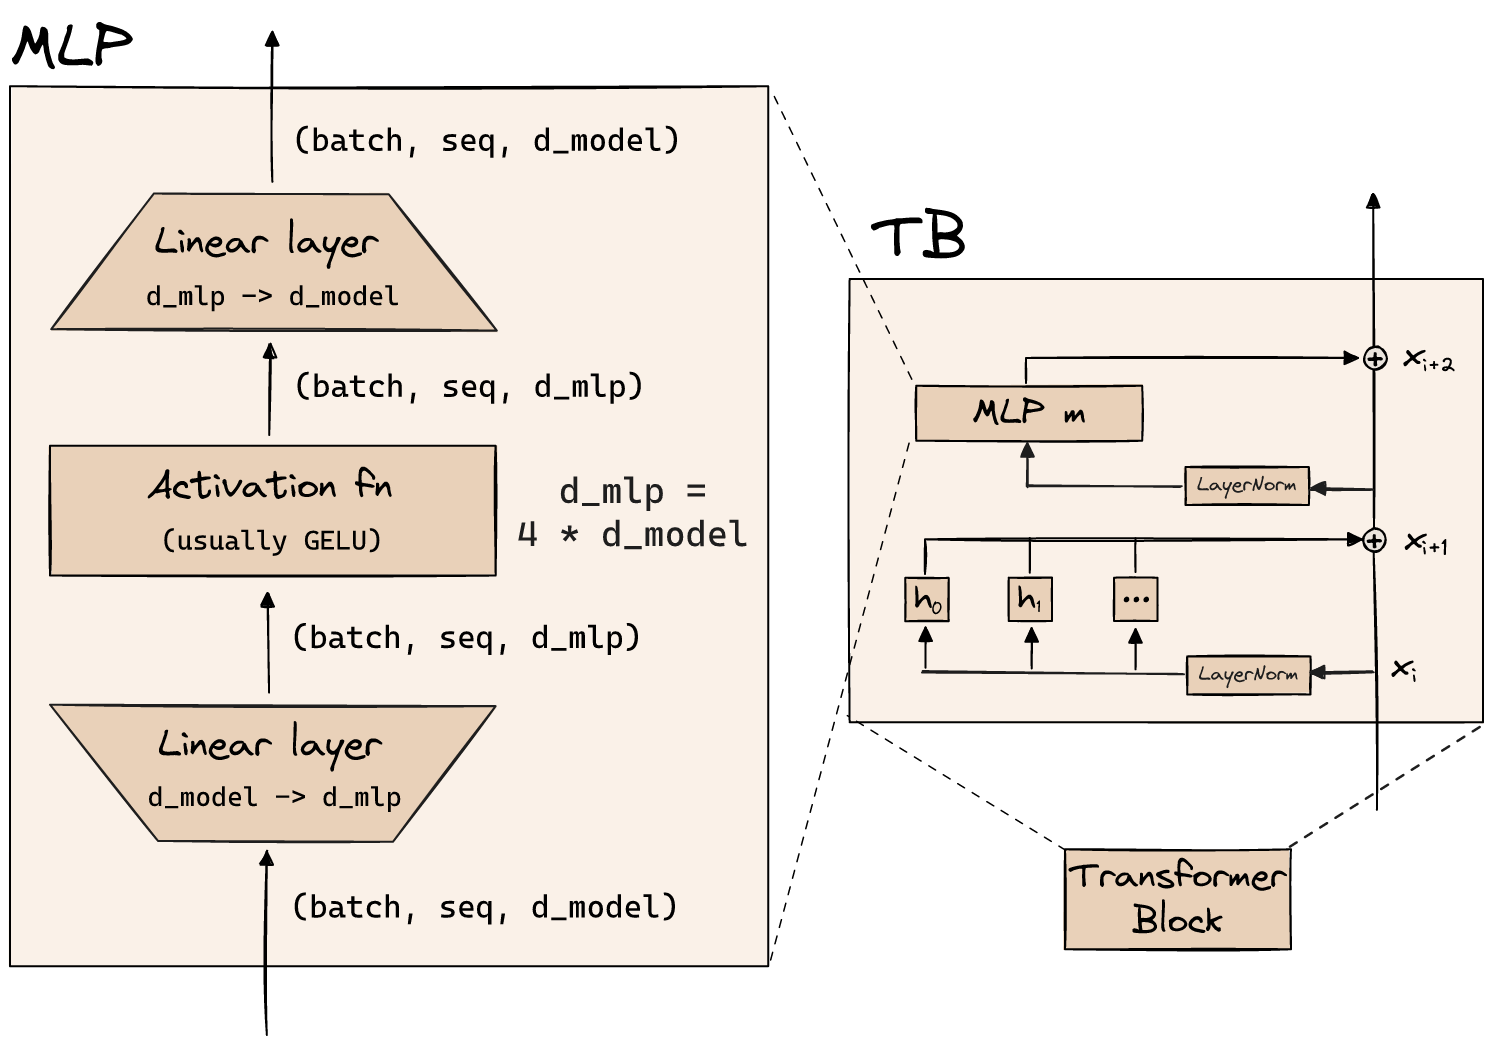
\includegraphics[width=0.75\linewidth]{MLP.png}
    \caption{MLP block inner structure \cite{colab_transformer_2024}}
\end{figure}

\subsection{Residual stream}
The residual stream is a critical concept in the Transformer architecture. It allows efficient gradient flow and knowledge accumulation across layers. Instead of completely replacing input embeddings at each step, the Transformer layers incrementally refine the input by adding modifications to the residual stream \cite{ferrando_primer_2024}. As there is no processing done in the residual stream, it can be considered as a channel of communication between the different components of the model \cite{nanda_mathematical_nodate}.

One key feature of its linear nature is the presence of "virtual weights," which establish indirect connections between layers even when separated by multiple intermediate layers. These virtual weights are computed by combining the output weights of one layer with the input weights of another, enabling efficient data retrieval from earlier layers. An example is $W_I^3W_O^1$ which is how layer 3 reads in the value from layer 1.

Due to the high dimensionality of the residual stream, it can store various types of information in distinct subspaces. This aspect is particularly important for attention heads, which work within relatively small subspaces, often around 64 to 128 dimensions. By writing data into separate subspaces, attention heads can operate independently without interference.

Stored information within the residual stream remains accessible unless explicitly removed or overwritten by subsequent layers. Thus, the dimensions of the residual stream can be seen as a form of memory or bandwidth. However, because there are far more computational elements, such as neurons and attention heads, compared to the available dimensions in the residual stream, bandwidth is in high demand. To manage this complexity, certain MLP neurons and attention heads seem to act as "memory managers" by clearing out data written by earlier layers \cite{nanda_mathematical_nodate}. They achieve this by reading stored values and writing their negative counterparts to free up space for new information. This process highlights the necessity of analysing virtual weights to understand information flow, rather than directly examining the residual stream.

\subsection{Layers}
Transformer models are composed of multiple stacked layers (residual blocks), each containing an attention block and an MLP block. Each layer refines the token representations progressively through:
\begin{itemize}
    \item Layer normalization, which helps stabilize training and ensures numerical consistency.
    \item Stacked attention and MLP layers, contributing to deeper feature learning as the layers progress.
    \item Final processing, where the accumulated residual stream is mapped to the output vocabulary space for prediction.
\end{itemize}

\section{Counterfactual explanations}
It is believed that \textit{causal understanding} is a necessary condition for satisfying the demand for XAI \cite{chou_counterfactuals_2022}. Philosophers generally agree that understanding why something is the case requires having true beliefs about what caused it \cite{baron_explainable_2023}. In the context of XAI, this means that in order to provide genuine explanatory understanding to users, the information delivered must accurately capture the causal factors that led a machine learning model to produce a particular output.
 
The counterfactual approach to XAI is seen as one of the central ways to meet this demand, as counterfactual explanations are intended to provide information about the causes underlying a model's output \cite{buijsman_defining_2022, miller_explanation_2019}. By specifying how a model's inputs would need to change in order to yield a different output, counterfactual explanations are supposed to reveal the causal dependencies at play making them a good approach to XAI \cite{baron_explainable_2023}.

The core idea is to find a minimally altered version of the input that changes the model's output. This contrastive approach aligns well with how humans naturally seek to understand events - not just why something happened, but why it happened instead of some alternative \cite{wachter_counterfactual_2017, celar_how_2023}.

Given an input $x$, and a binary classifier $\mathcal{M}$ such that $\mathcal{M}(x)=c$, A counterfactual explanation $x'$ is computed as \cite{karimi_survey_2023}:
\begin{equation}
   \arg \min_{x'} d(x',x)
    \label{eqn:closeness}
\end{equation}

\begin{equation}
    \text{subject to } \mathcal{M}(x') = 1-c
    \label{eqn:validity}
\end{equation}

Where $d$ is a distance function. Counterfactual explanations where \ref{eqn:validity} holds are known as \emph{valid} because they change the output class. \ref{eqn:closeness} can be relaxed to find counterfactuals that are \emph{close} to the original input but still valid, allowing for searching methods such as gradient descent.
 
Generating high-quality counterfactuals requires balancing three key properties: \cite{mcaleese_comparative_2024}
\begin{itemize}
    \item \textbf{Validity}: The counterfactual input must actually change the model's prediction, demonstrating the causal factors at play.
    \item \textbf{Sparsity}: The number of changes made to the original input should be minimized, highlighting the most influential features.
    \item \textbf{Plausibility}: The counterfactual must be a realistic input that falls within the model's expected distribution of inputs.
\end{itemize}

\subsection{Counterfactual explanations for textual data}
In the context of textual data, achieving this balance is non-trivial, as we are working on natural language instead of continuous data such as tabular data. Plausibility becomes more difficult as we want our counterfactual explanation to be a grammatically correct sentence but also have correct semantic meaning that is relevant and expected. Previous work has explored a variety of methods, from gradient-based techniques to approaches leveraging large language models. Understanding the strengths and limitations of these different approaches is important to understand what problems need to be solved so that complex NLP models can be more transparent and trustworthy.

\begin{figure}[h]
    \centering
    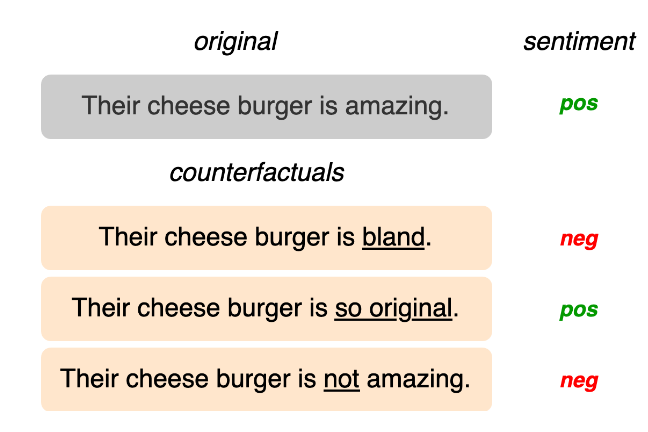
\includegraphics[width=0.5\linewidth]{ce_text.png}
    \caption{Examples of counterfactual explanations with opposing or similar labels for an example input sentence \cite{bhattacharjee_zero-shot_2024}}
    \label{fig:enter-label}
\end{figure}
 
By building on the foundations laid out in these prior works, this paper aims to develop a novel counterfactual explanation method that combines the best attributes of existing techniques to generate high-quality, informative and valid counterfactuals for text classifiers.
\subsubsection{Adversarial methods}
Adversarial examples are intentionally crafted inputs that cause models to make incorrect predictions with high confidence, despite being nearly indistinguishable from valid inputs to human observers. These examples are created by applying small, carefully calculated perturbations to legitimate input data until the classification changes \cite{goodfellow_explaining_2015}.

\begin{figure}[h]
    \centering
    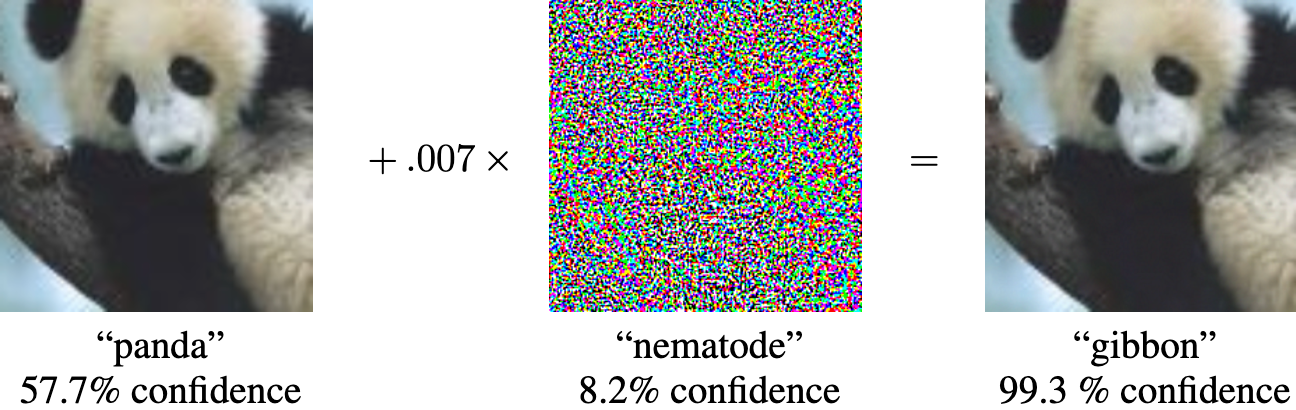
\includegraphics[width=0.7\linewidth]{adversarial.png}
    \caption{Example of an adversarial perturbation changing image classification score \cite{goodfellow_explaining_2015}}
    \label{fig:enter-label}
\end{figure}

Although these methods can be adapted to generate counterfactuals due to their ability to identify small changes that affect model outputs efficiently, they typically do not consider whether the modifications they produce are realistic or interpretable. As a result, when adversarial approaches are used to generate counterfactual explanations, they often create examples that, while mathematically valid, appear unnatural or implausible when evaluated.

An example is \textbf{HotFlip} \cite{ebrahimi_hotflip_2018}, a white-box method for generating adversarial examples for text classifiers by making minimal character-level changes to the input text. The key insight behind HotFlip is using gradient information from the model to identify the most impactful character changes that will cause misclassification.

HotFlip first generates a list of candidate substitutions for each position. It will then score these candidates with the calculated partial derivative of the output of the classifier with respect to the substitution. Next, using beam search, it iteratively builds upon the highest-impact candidates. At each step, we maintain a set of the top partial solutions within our budget and evaluate additional substitutions that could be made to each one. This process repeats until either the classifier's output changes or it exhausts all possible positions for substitution.

HotFlip aims to alter the classifier's output with minimal modifications, resulting in counterfactuals that typically achieve high scores in terms of validity and sparsity. However, as HotFlip does not account for the plausibility of its substitutions, the generated counterfactuals may exhibit low plausibility scores and may appear unnatural to human readers.


\subsubsection{Substitution methods}
Substitution methods, like adversarial methods, will identify important words for substitutions to keep the number of substitutions to change the classifier's output low. However, they also aim to generate plausible counterfactuals by making substitutions that keep the modified input plausible. Several earlier methods belong to this category, including REP-SCD \cite{yang_generating_2020}, MiCE \cite{ross_explaining_2021}, and CLOSS \cite{pope_text_2021}.
Taking a closer look at \textbf{CLOSS}, we define our problem as follows: 

Given an input token sequence $X=\{x_0,\dotsi,x_{n-1}\}$ and a classifier $\mathcal{M}$, with vocabulary $V$, with a binary class output $\hat{y}$. We aim to find a counterfactual $X'=\{x_0',\dotsi,x_{n-1}'\}$ such that $\mathcal{M}(X') \neq \hat{y}$ and $X'$ only differs from $X$ by some parameter of substitutions.

To generate candidate substitutions CLOSS first performs latent space optimization. As explained in section 2.2, our model $\mathcal{M}$ will map $X$ into embeddings $E=\{e_0,\dotsi,e_{n-1}\}$, we form an optimization equation:
\begin{equation}
    \min_{E'} CE(M(E'),y') + \sum_{j=0}^{n-1}|e_j'-e_j|
\end{equation}
Where $y'$ is the target class. This minimizes the cross-entropy between the model's output with the perturbed embedding $E'$ and the target class $y'$. We add a LASSO regularization term to favour sparse solutions. CLOSS only optimises $E'$ for K steps, considering each step. It then passes each $E_k'$ through a pre-trained model to get a logit matrix $T_k$ with dimensions $(|V| \times n)$. $T_k(s,t)$ is the likelihood of the $s$-th token of the vocabulary at token position $t$ in $E_k'$. Then it collects the $K$ best substitutions for each position $t$ into the set $S_t^k$ by iterating over $T_1$ to $T_k$, excluding any previous selections.

CLOSS then evaluates these substitutions by using Shapely values \cite{lundberg_unified_2017}. The Shapely value in this context represents the expected marginal value of adding the substitution $s$ into a set of substitutions without $s$ with maximum size $c_s$. Finally, to construct our counterfactual, it will perform beam search, by selecting substitutions with the highest Shapely values at each iteration.

\subsubsection{LLM methods}
As we have seen in substitution-based methods such as CLOSS, recent developments in large language models (LLMs) have transformed the landscape of counterfactual explanation generation for text classifiers. However, the use of the LLM was limited, and the architecture's inner workings were relied on, making them much less generalizable.

The field has evolved with the emergence of more LLM-centric approaches for counterfactual generation. The first category encompasses controlled generation techniques, exemplified by Polyjuice \cite{wu_polyjuice_2021} and GYC \cite{madaan_generate_2021}, which employ fine-tuned models to produce counterfactuals. \textbf{Polyjuice} is a controlled generation method for counterfactual explanations by fine-tuning GPT-2 with a prompt \cite{radford_language_2019}. Counterfactual generation was converted into a conditional text generation task. The prompt contained training data of the form $(x,c,\hat{x})$, as shown in \ref{fig:train_prompt}, where $x$ was the original input, $c$ was a control code, and $\hat{x}$ as the counterfactual. The control code specified what type of perturbation was wanted, \ref{fig:control_codes} lists all 6 types and examples of counterfactuals generated with these control codes. As you can see in line 3 \ref{fig:train_prompt}, it is fine-tuned to handle filling in \texttt{[BLANK]} tokens allowing for counterfactual generation at different granularities. Polyjuice accepts and input prompt with the lines 1-3 if specificity is needed however just line 1 is also fine as the LLM will just generate the control code and blank spaces.

\begin{figure}[h]
    \centering
    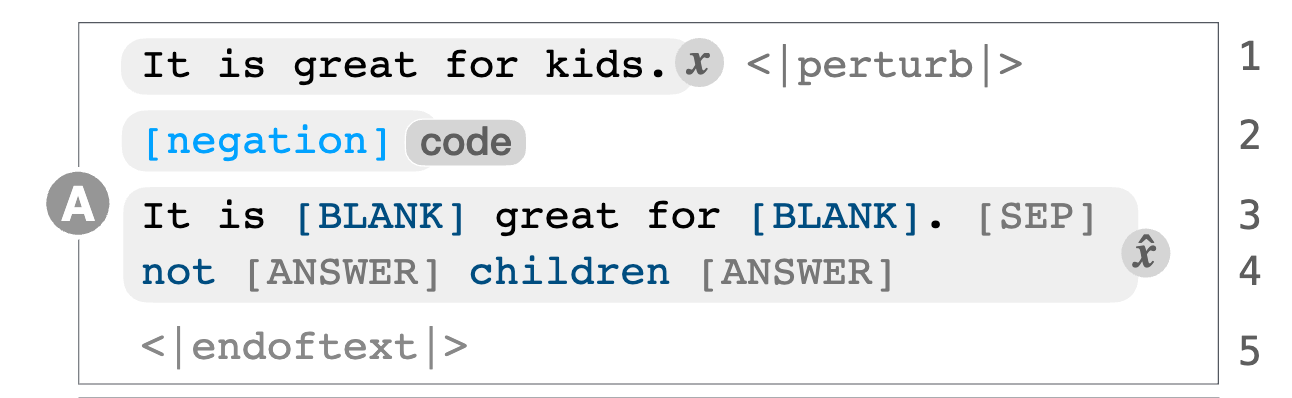
\includegraphics[width=0.7\linewidth]{polyjuice_train_prompt.png}
    \caption{Example of a training example \cite{wu_polyjuice_2021}}
    \label{fig:train_prompt}
\end{figure}

\begin{figure}[h]
    \centering
    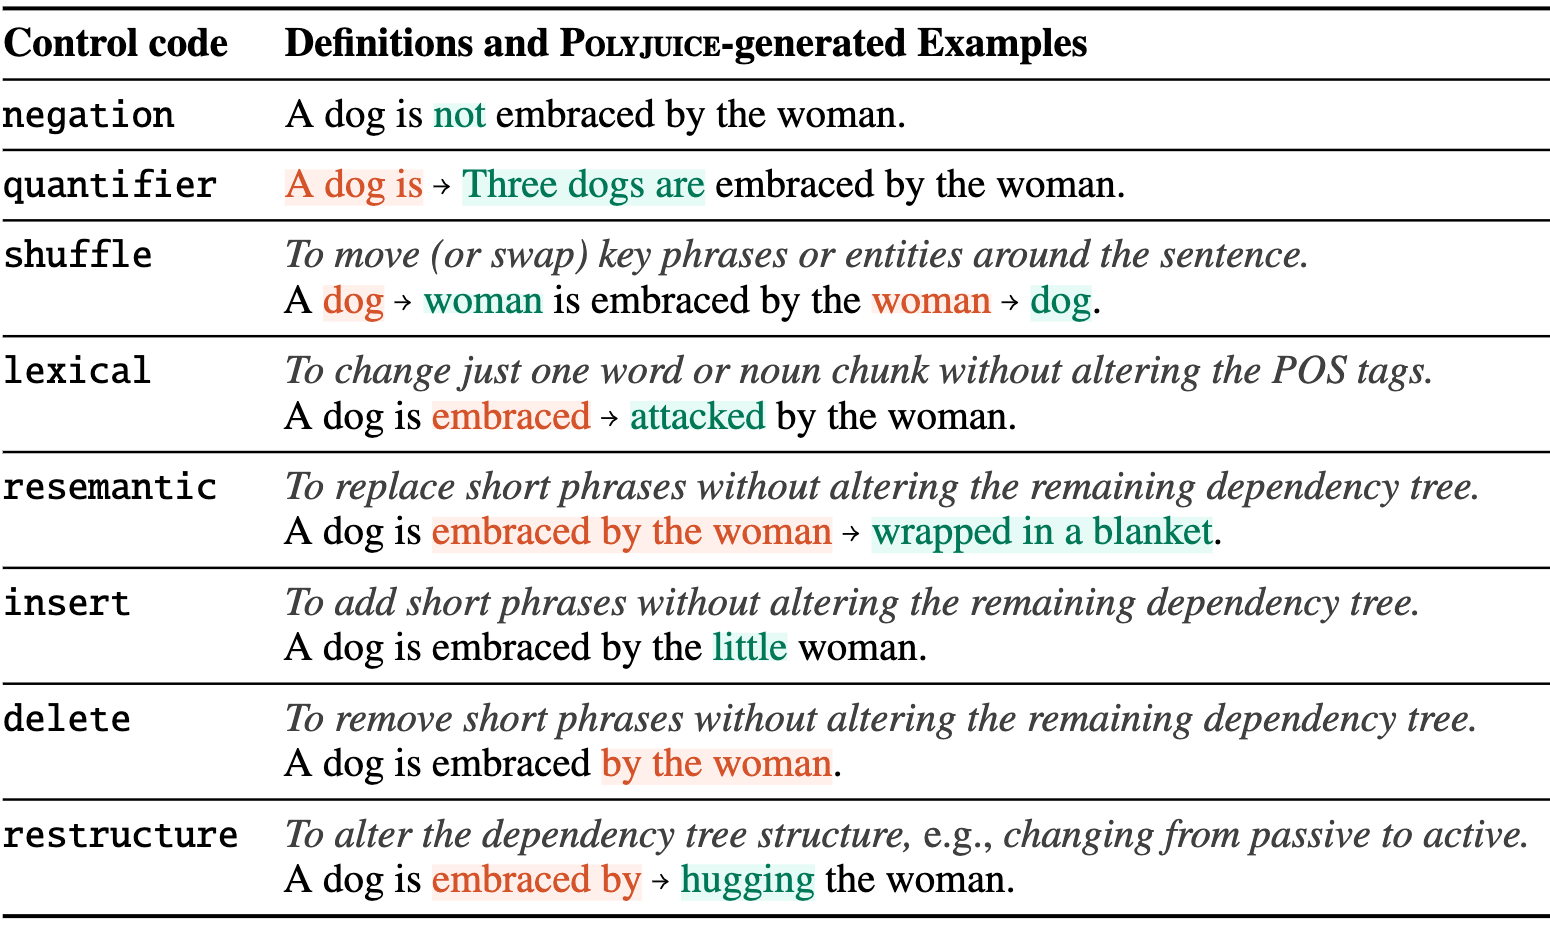
\includegraphics[width=0.85\linewidth]{control_codes.png}
    \caption{Table of control codes and example counterfactuals \cite{wu_polyjuice_2021}}
    \label{fig:control_codes}
\end{figure}

The second category consists of general-purpose LLM methods, such as FIZLE \cite{bhattacharjee_zero-shot_2024}. These methods use specifically crafted system prompts for counterfactual generation, eliminating the requirement for task-specific model adaptation through fine-tuning.
\subsubsection{Conclusion}

We can draw some important conclusions by analysing the evaluation of the mentioned methods from \ref{fig:ce_text_table}. We see HotFlip have the best similarity scores as it is an adversarial method, however, perplexity scores are also the highest meaning plausible counterfactuals are not produced. CLOSS performs the best in the flip score category across both datasets, with better perplexity scores than HotFlip due to the plausible substitution generation with a slight hit to similarity due to larger changes. LLM-based methods all have much lower perplexity scores but similarity scores do suffer and this may be because there is a trade-off between perplexity and similarity for LLM-based methods as the more control the LLM is given to change the original sentence, the more coherent the modified sentence will be as the LLM has more control. However, flip scores are very inconsistent and can get very low depending on the dataset signifying that even though realistic and correct counterfactuals are generated, they fail to flip the actual classification. This is probably due to not having access to any internal information on the model such as gradients. 
Other research has also shown that LLMs seem to produce very plausible explanations, however, these would not reflect the actual internal workings of the model \cite{atanasova_faithfulness_2023, parcalabescu_measuring_2024, turpin_language_2023} which explains the low and inconsistent flip scores despite the perplexity scores.

From the analysis, we can conclude that there are trade-offs based on the method and dataset used. So we aim to create some combination of these approaches to create a novel method that doesn't suffer from the drawbacks of a single approach.

\begin{figure}[ht]
    \centering
    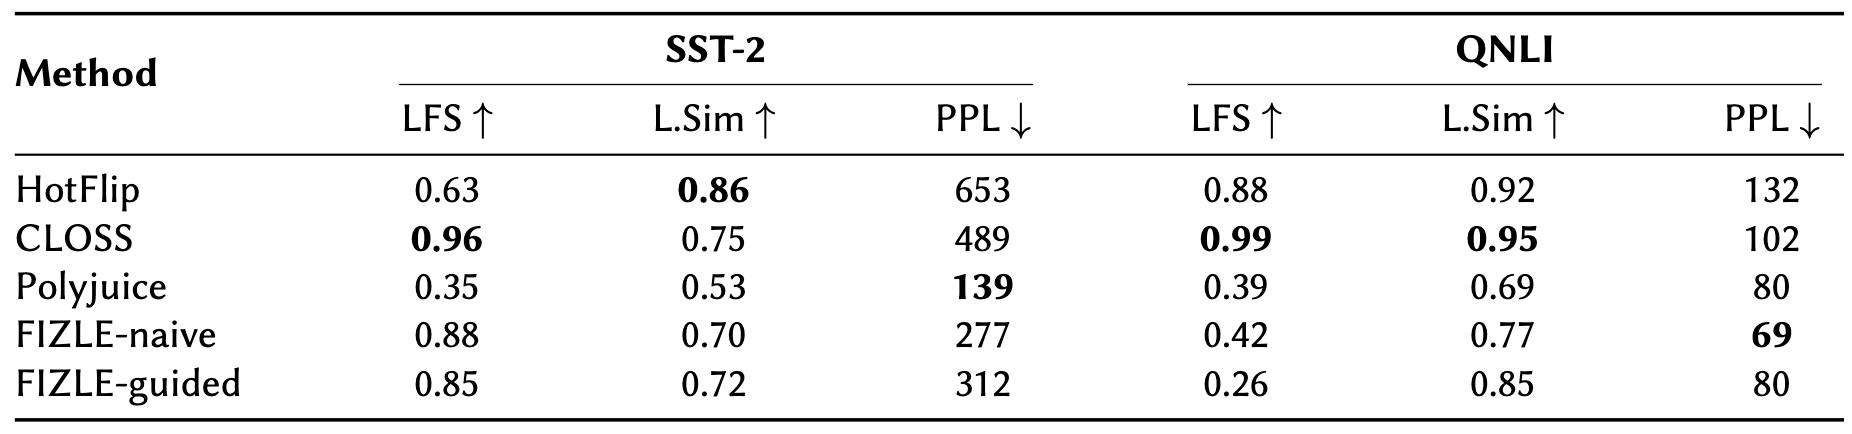
\includegraphics[width=1\linewidth]{ce_text_table.png}
    \caption{Comparison over evaluated scores for five counterfactual generation methods on two datasets. Label Flip Score (LFS), Levenshtein similarity (L.sim), and Perplexity (PPL) are the evaluated metrics \cite{mcaleese_comparative_2024}}
    \label{fig:ce_text_table}
\end{figure}

\newpage

\section{Mechanistic Interpretability}
With mechanistic interpretability, we aim to decode and understand parts of complex machine learning models by analysing and reverse-working their internal processes into some method or algorithm that gives some humanly understandable inspection of certain behaviours of the model \cite{geiger_causal_2021, wang_interpretability_2023}. This understanding can then be leveraged for a multitude of problems such as diagnosing and rectifying model errors \cite{vig_investigating_2020} or better aligning the model for its intended use case \cite{li_inference-time_2023}.

\subsection{Behaviour localisation}
Behaviour localisation refers to the process of identifying and "localising" the components within the model through a forward pass that are responsible for producing some behaviour or output \cite{ferrando_primer_2024}. For example, if an LLM consistently produces a biased response, behaviour localisation would attempt to locate the components that cause the undesired behaviour. We take a look at one type of method, i.e. \textit{input attribution}.

\subsection{Input attribution}
\textit{Input attribution} performs behaviour localisation by calculating the importance of each token in an input sequence $x$ in the resulting output \cite{ferrando_primer_2024}. We take a closer look at two such methods of approximation.

Gradients capture the sensitivity of the output with respect to some input token \cite{denil_extraction_2014}. We first calculate the gradient of the output with respect to each token embedding:
$$g(x_i)=\nabla_{x_i}q(y_t|\bm{x})$$
We can then calculate saliency scores by taking the $L1$ norm of the gradient at each $x_i$. However, it seems that these probabilities aren't too useful for understanding the model's decisions \cite{holtzman_surface_2021}. For example, most probability density is focused on semantically similar tokens. Instead of thinking why was $w$ predicted, we instead pose the problem as why was $\omega$ predicted \textit{instead of} $\sigma$. This is known as a contrastive explanation \cite{yin_interpreting_2022}. We can then build on our equation to \textit{Contrastive Gradient Norm} defined by:
$$g^*(x_i)=\nabla_{x_i}(q(y_t|\bm{x})-q(y_f|\bm{x}))$$ and then take the $L1$ norm again for saliency scores.

\begin{figure}[ht]
    \centering
    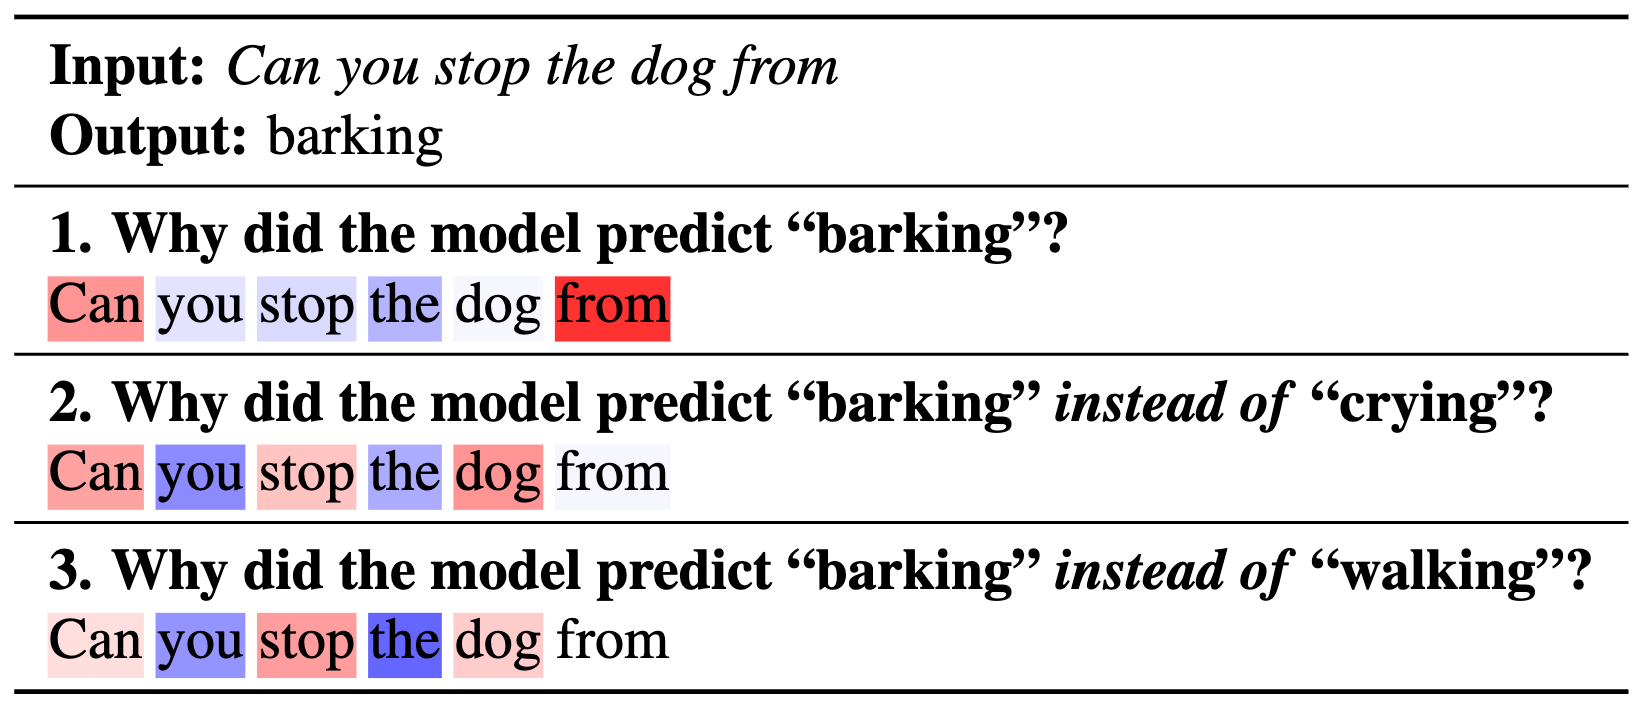
\includegraphics[width=0.75\linewidth]{contgrad.png}
    \caption{Explanations for next-word prediction. Blue means the token lowered the probability of the generated token and vice versa for red. (1) is a normal gradient-based explanation which doesn't provide much interpretable information. (2) is a contrastive explanation and hints that the "dog" token caused it to pick the verb more relevant to dogs, "barking" (3) hints that the "stop" token caused it to pick the more negatively viewed verb "barking" as compared to "walking"}
    \label{fig:enter-label}
\end{figure}

\newpage

\subsection{Patchscopes}
Activation patching is an existing idea for \textit{causal intervention} \cite{geiger_causal_2021}, used to localise components of the model that contribute to the output \cite{stolfo_mechanistic_2023} and for detecting circuits, which are groups of model components that interact together via the residual stream to solve a task \cite{wang_interpretability_2023, cammarata_thread_2020}. The idea proposed by Patchscopes \cite{ghandeharioun_patchscopes_2024} is to take this a step further than localisation and to extract encoded information from specific activations and "translate" it into natural language text by leveraging an LLM. It aims to guarantee that no further information from the source context is encoded due to patching the activation into a different context.

With a source prompt $S$ of $n$ tokens, and a model $\mathcal{M}$ of $L$ layers, $\bm{h}_i^l$ is the activation for token $i$ at layer $l$ in $\mathcal{M(S)}$. We then take a separate forward pass on a model $\mathcal{M^*}$ of $L^*$ layers, on a target prompt $T$ of $m$ tokens. We choose some activation $\bar{\bm{h}}_{i^*}^{l^*}$ from $M^*(T)$. We then perform patching by applying $\bar{\bm{h}}_{i^*}^{l^*} \xleftarrow{} f(\bm{h}_i^l)$ where $f$ is defined as a mapping function $f(\bm{h};\bm{\theta}):\mathbb{R}^d \xrightarrow{} \mathbb{R}^{d^*}$. The Patchscope operation on $(S, i, \mathcal{M}, l)$ is defined by $(T,i^*,f,\mathcal{M}^*,l^*)$. The $f$ function is very flexible where it could just be the identity function or have a more complex definition.

\begin{figure}[h]
    \centering
    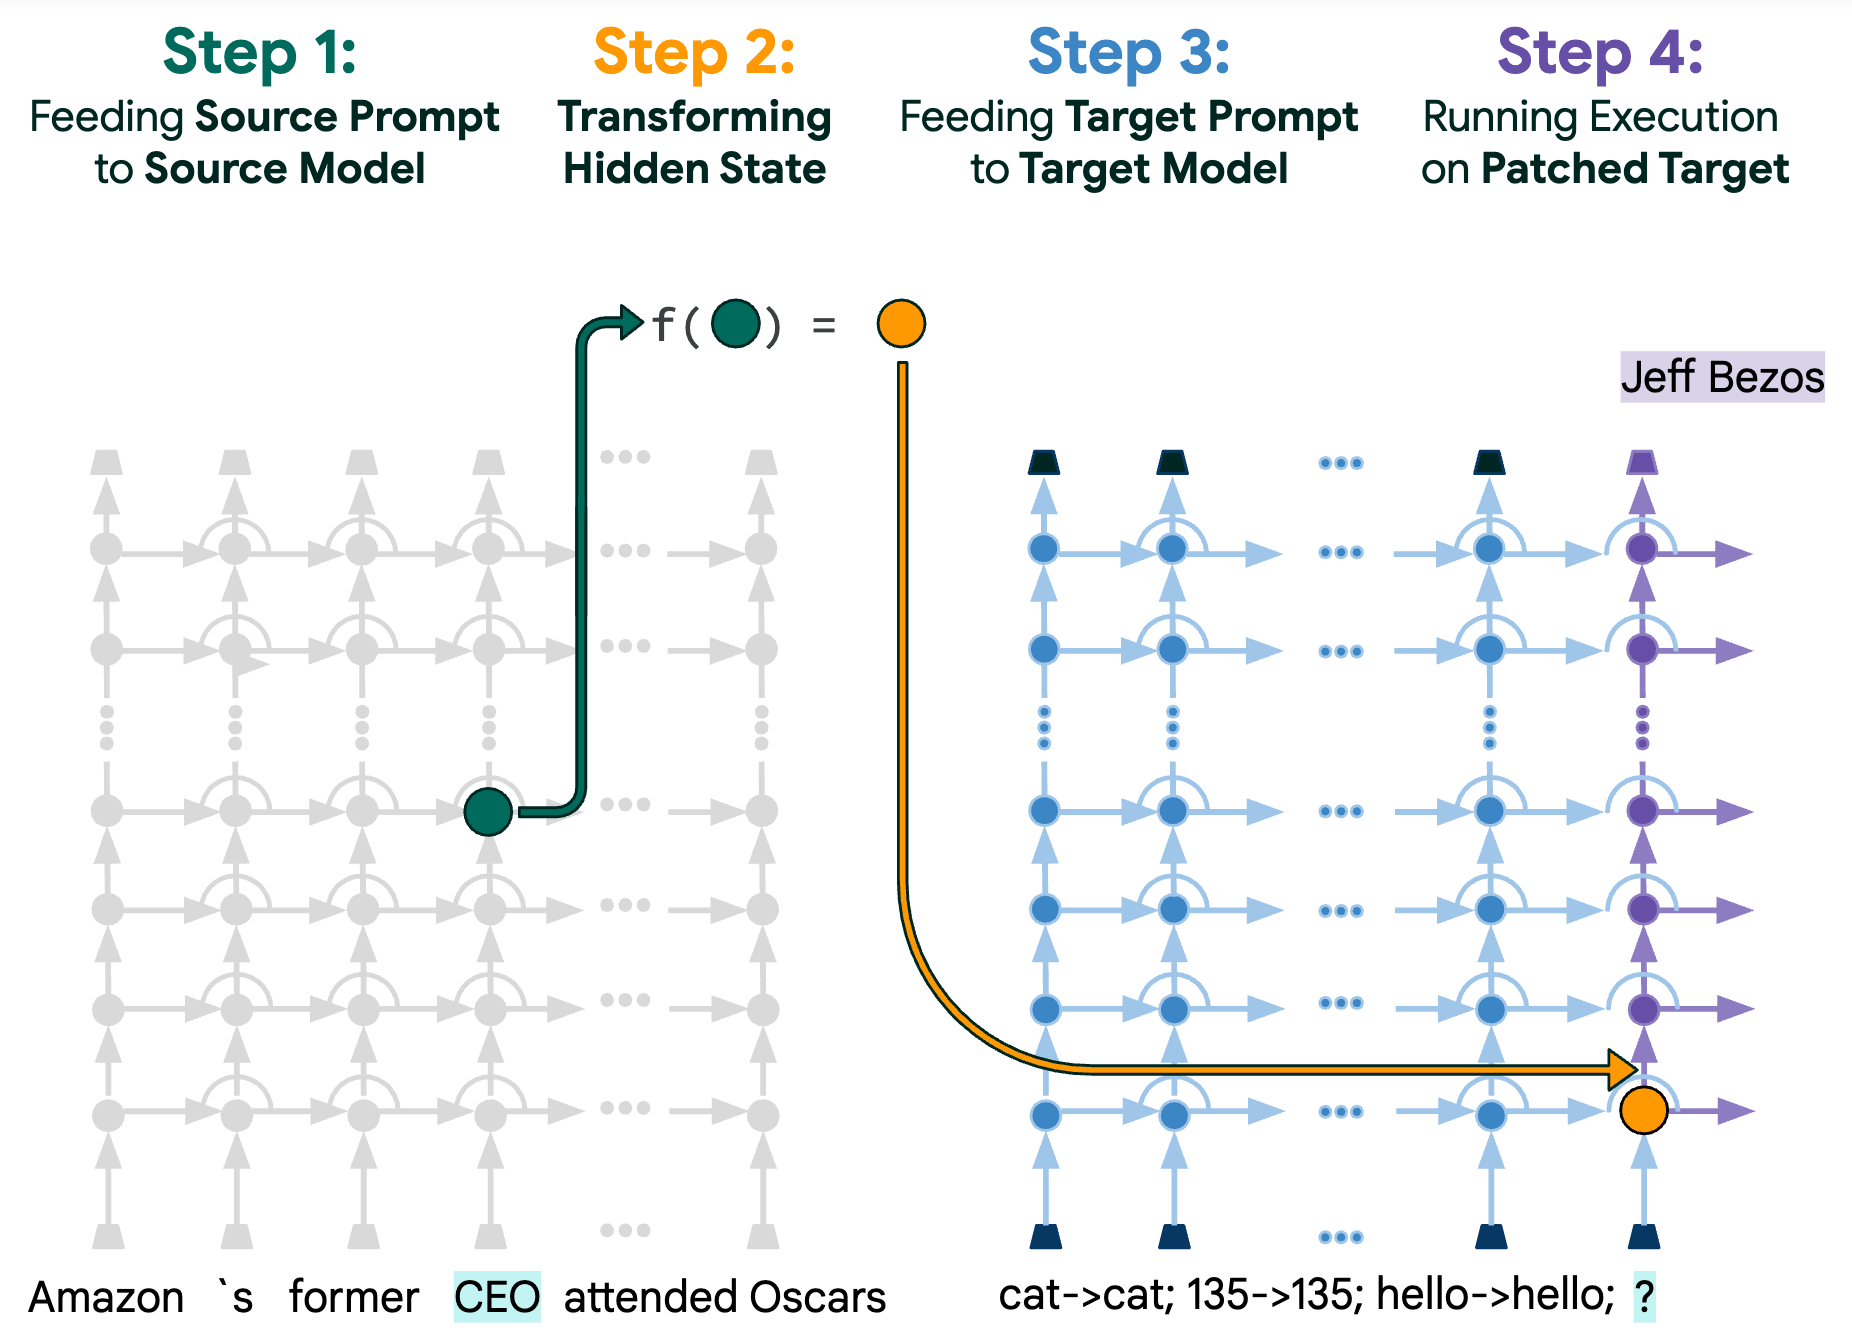
\includegraphics[width=0.95\linewidth]{patchscopes.png}
    \caption{An example of a Patchscope, where the activation of "CEO" at some layer has had its token representation decoded by a target prompt $T$ that encourages the LLM to output this. In this case, we get "Jeff Bezos" \cite{ghandeharioun_patchscopes_2024}}
    \label{fig:enter-label}
\end{figure}

The draw of Patchscopes is that across multiple inspection objectives, it can express existing methods through a configuration of Patchscopes and even improve upon them with new configurations due to the robustness and expressiveness provided by the framework. This is shown in table \ref{fig:patchscopes_configs}.

\textbf{Next-token prediction} The goal is to estimate the output probability distribution $\bm{p}^L$ from a hidden representation $\bm{h}^l$ across the models layers. This helps us understand how early the model has calculated its final prediction from the input. As discussed before, different lens such as \textit{Logit Lens} \cite{nostalgebraist_interpreting_2020}, and \textit{Tuned Lens} \cite{belrose_eliciting_2023} are methods for this inspection. Both of these can be represented as Patchscope configurations. However, we propose \textit{Token Identity} which uses a few-shot target prompt $T=\text{"}tok_1\xrightarrow{}tok_1;tok_2\xrightarrow{}tok_2;\dotsi;tok_k\text{"}$ to help encourage the LLM in decoding the token representation of the activation. The evaluation results show \textit{Token Identity} mostly outperforming other methods across the board with higher precision and lower surprisal scores across the layers except near the starting layers where it performs on-par or slightly worse whilst not requiring any train step.

\textbf{Extraction of specific attributes}
For a subject $\sigma$, a relation $\rho$, and an object $\omega$, we wish to see if the object $\omega$ is encoded in the representation of $\sigma$ in some arbitrary context. For example for the subject "United States" we want to see if "New York City", as the object, is encoded in the subject as they are related by the relation "largest city of". This is usually done by some method of probing \cite{belinkov_probing_2022}. However, these need to be pre-trained and consequentially the output classes must be pre-defined making this method quite rigid, so we propose a Patchscope configuration that does not face these limitations with a zero-shot prompt approach. $S$ remains the same as the input prompt with $\sigma$ in some arbitrary context. However, $T$ is a formulation of $\rho$ in a way that we can form a natural sentence in the order $\rho \xrightarrow{} \sigma \xrightarrow{} \omega$, where we replace $\sigma$ with a single arbitrary token such as $x$ and omit $\omega$. For our previous example, $T$ = "The largest city of $x$". We form it this way so that $i^*$ will be the last token $x$. $i$ is the last token of $\sigma$ in $S$. We finally check for any mention of $\omega$ in the generated output from $M^*$. Evaluating this against a logistic regression probe \cite{kohn_whats_2015, gupta_distributional_2015} we see the general trend is that the Patchscope outperforms in lower layers, is on-par in middle layers and performs worse in later layers.

Conclusively we see that Patchscopes is a simple but powerful framework for performing interpretability over LLMs and that existing methods only range a small subset of possible configurations, with unexplored configurations hopefully helping decode some arbitrary information to help engineer a novel method of generating plausible yet valid counterfactual explanations.

\begin{figure}[ht]

    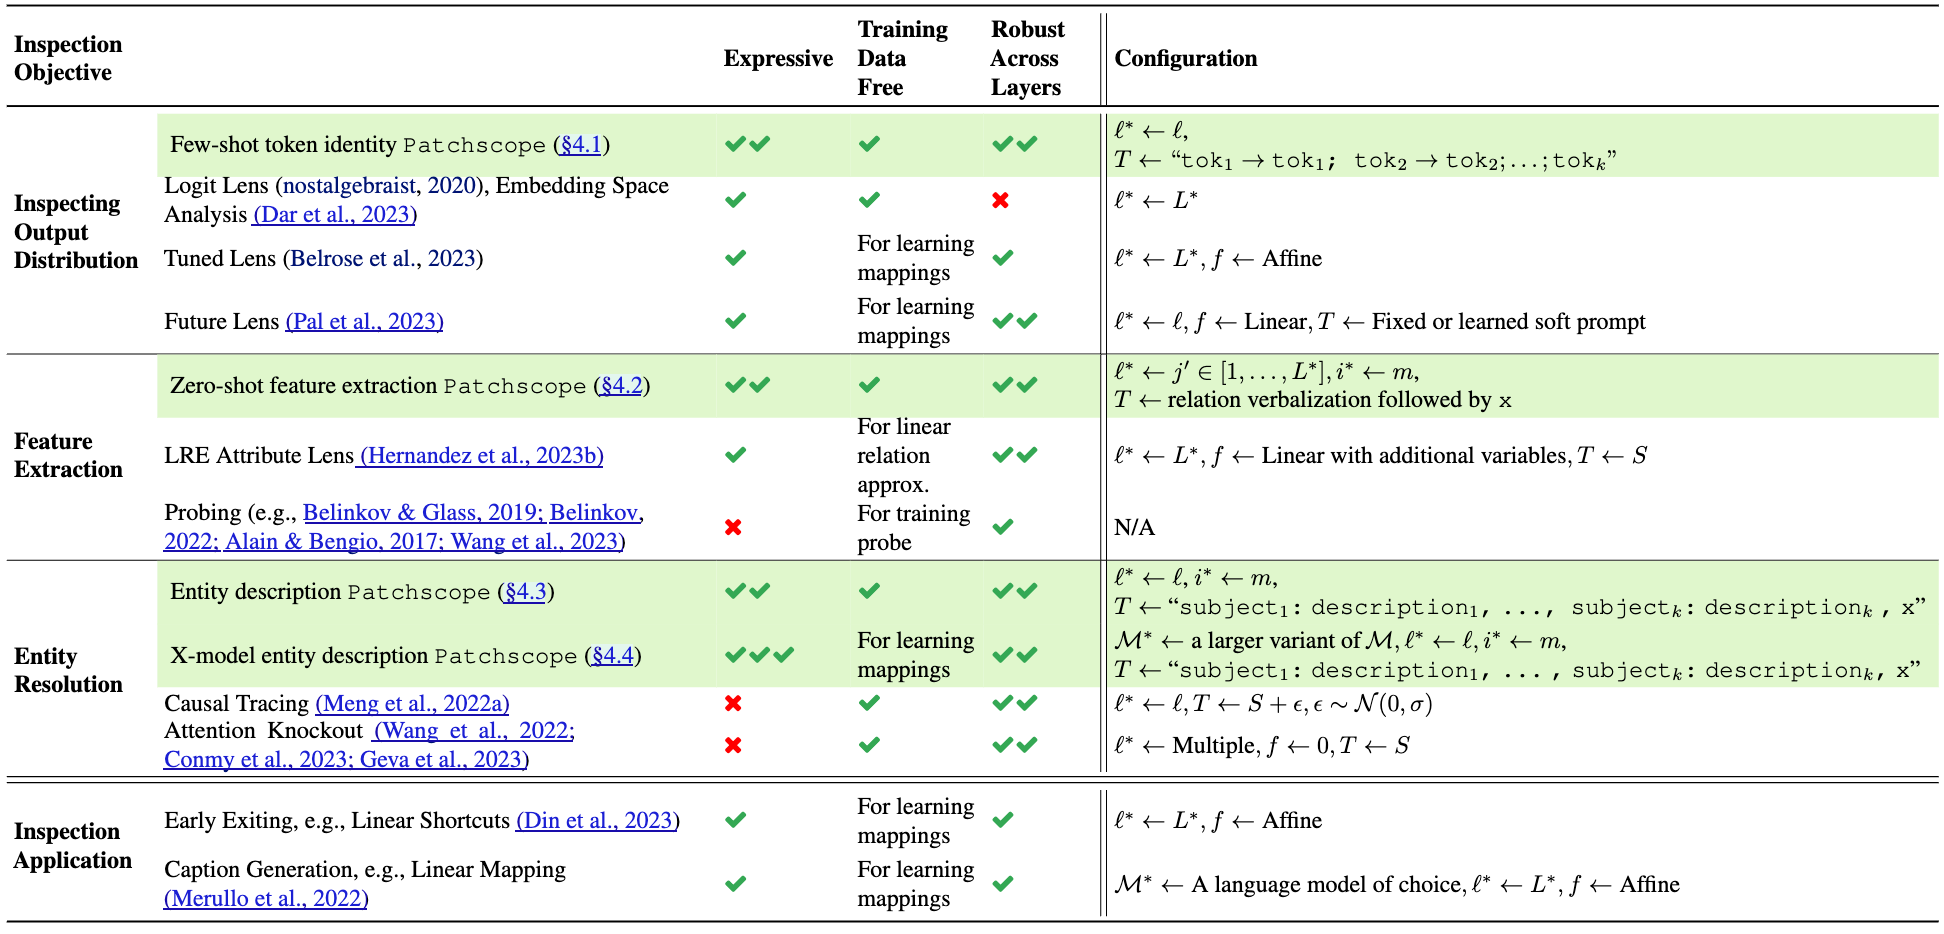
\includegraphics[width=1\linewidth]{patchscopes_configs.png}
    \caption{The table shows configurations of Patchscopes that emulate other inspection methods and new configurations in green that improve upon them \cite{ghandeharioun_patchscopes_2024}}
    \label{fig:patchscopes_configs}
\end{figure}
